\subsection{紧空间与局部紧空间的商空间}

命题 8. 设 X 是紧空间，R 是 X 上的一个等价关系，C 是 R 在 X × X 中的图象，f 是典范映射 X → X/R。则以下条件等价：

\begin{enumerate}
\def\labelenumi{\alph{enumi})}
\item
  C 在 \(\mathbf{X} \times \mathbf{X}\) 中是闭的。
\item
  R 是闭的。
\item
  \(f\) 是逆紧的。
\item
  X/R 是豪斯多夫的。
\end{enumerate}

此外，若这些条件满足，则 X/R 是紧的。

R 是闭的当且仅当 \(f\) 是闭的；故由第 2 目定理 1 b)，b) 蕴含 c)。c) 蕴含 d) 是第 1 目命题 5 推论 2 的特殊情形。对任意拓扑空间 \(\mathbf{X}\)，d) 蕴含 a)（\(\S 8\)，第 3 目，命题 8）。剩下要证 a) 蕴含 b)。若 \(\mathbf{F}\) 是 \(\mathbf{X}\) 的一个闭子集，它的（关于 \(\mathbf{R}\) 的）饱和集是 \(\mathrm{pr}_2(\mathbf{C} \cap (\mathbf{F} \times \mathbf{X}))\)；由假设，\(\mathbf{C} \cap (\mathbf{F} \times \mathbf{X})\) 是紧空间 \(\mathbf{X} \times \mathbf{X}\) 的一个闭子集，因而是紧的（\(\S 9\)，第 3 目，命题 3）；结论由 \(\mathrm{pr}_2\) 的连续性得出（\(\S 9\)，第 4 目，定理 2，推论 2）。

最后，显然若 X/R 是豪斯多夫的，则它是紧的（§ 9，第 4 目，定理 2）。

命题 9. 设 X 是局部紧空间，R 是 X 上的一个等价关系，C 是 R 在 X × X 中的图象，f 是典范映射 X → X/R；设 X' 是由 X 添加无穷远点 ω 而得到的紧空间，R' 是 X' 上的图象为 C' = C ∪ \{(ω, ω)\} 的等价关系。则以下条件等价：

\begin{enumerate}
\def\labelenumi{\alph{enumi})}
\item
  \(f\) 是逆紧的。
\item
  X 的每个紧子集关于 R 的饱和集是紧的。
\item
  \(\mathbf{R}'\) 是闭的。
\item
  \(\mathbf{pr}_2\) 在 \(\mathbf{C}\) 上的限制是逆紧的。
\item
  R 是闭的且关于 R 的诸等价类是紧的。
\end{enumerate}

此外，若这些条件满足，则 X/R 是局部紧的。

\begin{enumerate}
\def\labelenumi{\alph{enumi})}
\item
  \(\Longrightarrow\) b)：由于 \(\mathbf{X} / \mathbf{R} = f(\mathbf{X})\) 且 \(f\) 是逆紧的，\(\mathbf{X} / \mathbf{R}\) 是豪斯多夫的（第 1 目，命题 5，推论 2）；故 \(f\) 下任意紧子集 \(\mathbf{K}\)（\(\mathbf{X}\) 的）的象是紧的（§ 9，第 4 目，定理 2，推论 1）。\(\mathbf{K}\) 关于 \(\mathbf{R}\) 的饱和集是 \(\overline{f}^1(f(\mathbf{K}))\)，因此由第 2 目命题 6 是紧的。
\item
  \(\Longrightarrow\) c)：若 \(F'\) 在 \(X'\) 中是闭的且不含 \(\omega\)，则 \(F'\) 是 \(X\) 的一个紧子集；故它关于 \(R'\) 的饱和集（即它关于 \(R\) 的饱和集）是紧的，从而更是在 \(X'\) 中闭的。若 \(\omega \in F'\) 且 \(F = F' \cap X = F' - \{\omega\}\)，则 \(F'\) 关于 \(R'\) 的饱和集是 \(\{\omega\}\) 与饱和集 \(H\)（即 \(F\) 关于 \(R\) 的饱和集）之并；故只须证明 \(H\) 在 \(X\) 中是闭的（即 \(R\) 是一个闭关系）。为此，只须证明对任意紧子集 \(K\)（\(X\) 的），\(H \cap K\) 是紧的（\(\S 9\)，第 7 目，命题 11）。现在饱和集 \(L\)（即 \(K\) 关于 \(R\) 的饱和集）由假设是紧的，而 \(H \cap L\) 是 \(F \cap L\) 的饱和集，它也是紧的；从而 \(H \cap K = (H \cap L) \cap K\) 更是紧的。
\item
  \(\Longrightarrow\) d)：由于 \(\mathbf{X}'\) 是正则的（§ 9，第 2 目，命题 1 的推论），\(\mathbf{C}'\) 在 \(\mathbf{X}' \times \mathbf{X}'\) 中是闭的（§ 8，第 6 目，命题 14），因而是紧的。由此推出 \(\mathbf{C}'\) 是 \(\mathbf{C}\) 的单点紧化（§ 9，第 8 目，定理 4）。由于 \(\mathbf{C}'\) 上 \(\mathrm{pr}_2: \mathbf{X}' \times \mathbf{X}' \to \mathbf{X}'\) 的限制在 \(\omega\) 处连续，结论由第 3 目命题 7 的推论得出。d) \(\Longrightarrow\) e)：若 \(\mathbf{F}\) 是 \(\mathbf{X}\) 的任意闭子集，则 \(\mathbf{C} \cap (\mathbf{F} \times \mathbf{X})\) 在 \(\mathbf{C}\) 中是闭的，于是 \(\mathbf{F}\) 关于 \(\mathbf{R}\) 的饱和集（它等于 \(\mathrm{pr}_2(\mathbf{C} \cap (\mathbf{F} \times \mathbf{X}))\)）在 \(\mathbf{X}\) 中是闭的（第 1 目，命题 1）。又 \(x \in \mathbf{X}\) 模 \(\mathbf{R}\) 的等价类同胚于 \(\{x\}\) 在 \(\mathrm{pr}_2\) 到 \(\mathbf{C}\) 的限制下的逆像，因此是紧的{[}第 2 目，定理 1 b){]}。
\item
  \(\Rightarrow\) a)：若 R 是闭的，则由定义 \(f\) 是闭的，且对每个 \(z \in \mathbf{X} / \mathbf{R}\)，\(\overline{f}^1(z)\) 是模 R 的一个等价类，因此是紧的；故由第 2 目定理 1 b)，\(f\) 是逆紧的。
\end{enumerate}

最后我们必须证明 X/R 是局部紧的。由 c) 与命题 8，\(X^{\prime}/R^{\prime}\) 是紧的；关系 R 是 \(R^{\prime}\) 在 X 上诱导的关系；X 在 \(X^{\prime}\) 中是开的且关于 \(R^{\prime}\) 是饱和的；故 X/R 同胚于象 \(f^{\prime}(X)\)（X 在典范映射 \(f^{\prime}: X^{\prime} \to X^{\prime}/R^{\prime}\) 下的）（§ 3，第 6 目，命题 10，推论 1）。而 \(f^{\prime}(X)\) 在 \(X^{\prime}/R^{\prime}\) 中是开的，因而是 \(X^{\prime}/R^{\prime}\) 的一个局部紧子空间。

证毕。

推论. 设 X 是豪斯多夫空间，Y 是拓扑空间，\(f: X \rightarrow Y\) 是逆紧映射。则 X 是紧的（相应地，局部紧的）当且仅当 \(f(X)\) 是紧的（相应地，局部紧的），且 Y 是紧的（相应地，局部紧的）便为充分。

若 X 是紧的（相应地，局部紧的），则 \(f(\mathbf{X})\) 是紧的（相应地，局部紧的）这一事实是第 1 目命题 5 推论 4 及命题 8 与命题 9 的推论（X 是紧的情形也是第 1 目命题 5 推论 2 及 § 9 第 4 目定理 2 的推论）。反之，若 \(Z = f(\mathbf{X})\) 是紧的（相应地，局部紧的），则由于

\(f_{\mathbf{Z}}: \mathbf{X} \to f(\mathbf{X})\) 是逆紧的{[}第 1 目，命题 3 a){]}，由第 2 目命题 6 与第 3 目命题 7 推出 \(\mathbf{X}\) 是紧的（相应地，局部紧的）。最后，若 \(\mathbf{Y}\) 是紧的（相应地，局部紧的），则 \(f(\mathbf{X})\)（它在 \(\mathbf{Y}\) 中是闭的；第 1 目，命题 1 及 § 9，第 7 目，命题 13）也是紧的（相应地，局部紧的）。

\pandocbounded{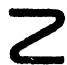
\includegraphics[keepaspectratio]{images/part001_1db83a62.jpg}}

注. 若 X 是局部紧的但不是紧的，则 X 上的闭等价关系 R 未必是豪斯多夫的（第九章，§ 4，习题 14）；而且即使 R 是豪斯多夫的，X/R 也未必是局部紧的（习题 17）。但我们有下述判别准则：

命题 10. 设 X 是局部紧空间，R 是 X 上的一个开的豪斯多夫等价关系，\(f: \mathrm{X} \to \mathrm{X}/\mathrm{R}\) 是典范映射。则 \(\mathrm{X}/\mathrm{R}\) 是局部紧的，且若 \(\mathbf{K}'\) 是 \(\mathrm{X}/\mathrm{R}\) 的任意紧子集，则存在 X 的紧子集 K，使得 \(f(\mathbf{K}) = \mathbf{K}'\)。

第一个断言是如下事实的推论：每个 \(x \in \mathbf{X}\) 有一个紧邻域 \(\mathbf{V}\)，且 \(f(\mathbf{V})\) 是 \(f(x)\) 的一个紧邻域（\(\S 5, \text{no. } 3, \text{ Proposition } 5\) 与 \(\S 9, \text{ no. } 4, \text{ Theorem } 2, \text{ Corollary } 1\)）。对每个 \(y \in \mathbf{K}'\)，设 \(\mathbf{V}(y)\) 是 \(\overline{f}^1(y)\) 的某个点在 \(\mathbf{X}\) 中的一个紧邻域，于是 \(f(\mathbf{V}(y))\) 是 \(y\) 的一个紧邻域。存在有限多个点 \(y_i \in \mathbf{K}'\)，使得诸 \(f(\mathbf{V}(y_i))\) 覆盖 \(\mathbf{K}'\)。设 \(\mathbf{K}_1\) 是紧集 \(\bigcup_i \mathbf{V}(y_i)\)（\(\mathbf{X}\) 中的）；我们有 \(\mathbf{K}' \subset f(\mathbf{K}_1)\)；故 \(\mathbf{K} = \mathbf{K}_1 \cap \overline{f}^1(\mathbf{K}')\) 是紧的（因为它在 \(\mathbf{K}_1\) 中是闭的），且 \(f(\mathbf{K}) = \mathbf{K}'\)。

